\documentclass{beamer}
\usepackage[english]{babel}
\usepackage{graphicx}
\usepackage{booktabs}
\usepackage{xcolor}
\usepackage{tikz}
\usetikzlibrary{positioning,arrows.meta}
\usepackage{hyperref}

% Customize bullet points
\setbeamertemplate{itemize items}[circle]
\setbeamertemplate{itemize subitem}[circle]

\title{Fine-tuning GPT-2 for Short Query Intent Classification}
\author{Jin Young Lee}
\date{\today}

\begin{document}

% Slide 1: Title
\begin{frame}
\titlepage
\end{frame}

% Slide 2: Search Intent Overview (New Slide)
\begin{frame}
\frametitle{Understanding Search Intent}
\centering
\begin{figure}
    \includegraphics[width=0.8\textwidth]{assets/search_intent.png}
    \caption{Different types of Search Intent}
\end{figure}
\end{frame}

% Slide 3: Motivation and Problem Statement
\begin{frame}
  \frametitle{Motivation and Problem Statement}
  \textbf{What is the problem? Why is it important?}
  \begin{itemize}
    \item Short queries (\texttt{e.g., "weather?", "pizza nearby"}) are ambiguous
    \item Misclassified intents degrade user experience
    \item Accurate intent classification is crucial for:
    \begin{itemize}
      \item Voice Assistants
      \item Search Engines
    \end{itemize}
    \item \textbf{Challenge:} Minimal context in short queries
  \end{itemize}
\end{frame}

% Slide 4: Proposed Approach and Methodology
\begin{frame}
\frametitle{Proposed Approach and Methodology}
\centering
\begin{tabular}{l p{0.6\textwidth}}
\toprule
\textbf{Category} & \textbf{Detail} \\
\midrule
\textbf{Model} & GPT-2 base model (768d hidden) \\
\textbf{Classification Head} & Custom linear layer \\
\textbf{Fine-tuning Modes} & Last-linear-layer, Full-model \\
\textbf{Regularization} & Dropout (0.3) \\
\midrule
\textbf{Optimizer} & AdamW \\
\textbf{Learning Rate} & 1e-3 \\
\textbf{Batch Size} & 8 \\
\textbf{Loss Function} & Cross-entropy \\
\textbf{Early Stopping} & Based on dev accuracy \\
\bottomrule
\end{tabular}
\end{frame}

% New Slide 5: Amazon MASSIVE Dataset Details (Previously part of Slide 5)
\begin{frame}
  \frametitle{Amazon MASSIVE Dataset (EN-US Subset)}

  {\footnotesize \href{https://huggingface.co/datasets/SetFit/amazon_massive_intent_en-US}{[View on Hugging Face]}}
  \vspace{1em}

  \centering
  \begin{tabular}{ll}
  \toprule
  \textbf{Feature} & \textbf{Description} \\
  \midrule
  \textbf{Total Languages} & 51 (Multilingual) \\
  \textbf{Subset Used} & \texttt{en-US} only \\
  \textbf{Utterance Count} & $\sim$60,000 utterances (EN-US) \\
  \textbf{Intent Classes} & 60 distinct intent types \\
  \textbf{Domains} & Music, Weather, Alarms, Smart Home, etc. \\
  \textbf{Utterance Length} & Mix of short and long queries \\
  \textbf{Label Quality} & Human-annotated, high quality \\
  \textbf{Source} & Amazon Alexa / MASSIVE Dataset \\
  \bottomrule
  \end{tabular}
  
\end{frame}

\begin{frame}
  \frametitle{MASSIVE Dataset: EN-US Subset Examples}
  
  \vspace{0.5em}
  \centering
  \scriptsize
  \begin{tabular}{cll}
  \toprule
  \textbf{ID} & \textbf{Utterance} & \textbf{Intent Label} \\
  \midrule
  1   & wake me up at nine am on friday     & alarm\_set \\
  2   & set an alarm for two hours from now & alarm\_set \\
  5   & stop                                & audio\_volume\_mute \\
  9   & make the lighting bit more warm here & iot\_hue\_lightchange \\
  15  & turn off the light in the bathroom  & iot\_hue\_lightoff \\
  22  & dim the lights in the kitchen       & iot\_hue\_lightdim \\
  25  & olly clean the flat                 & iot\_cleaning \\
  33  & check when the show starts          & calendar\_query \\
  34  & i want to listen arijit singh song once again & play\_music \\
  \bottomrule
  \end{tabular}
  \vspace{1em}
  
  \textit{Intent types include alarms, smart lighting, music playback, and calendar access.}
  \end{frame}

% New Slide 6: Data Preprocessing Pipeline - Input Example
\begin{frame}
\frametitle{Data Preprocessing Pipeline - Input Example}
\textbf{Preprocessing Steps for GPT-2:}
\begin{itemize}
  \item Tokenize input using GPT-2 tokenizer (BPE-based)
  \item Apply dynamic padding within batch
  \item Truncate to max model input length (e.g., 128)
  \item Use \texttt{<|endoftext|>} as padding token
  \item Track unique utterance ID for evaluation alignment
\end{itemize}
\vspace{1em}
\textbf{Example Utterance:}
\begin{itemize}
    \item \textbf{Text:} ``play some jazz music''
    \item \textbf{Intent:} \texttt{music.play\_song}
\end{itemize}
\end{frame}

% New Slide 7: Data Preprocessing Pipeline - Tokenization
\begin{frame}
  \frametitle{Tokenization Flow: From Text to Embeddings}
  \centering
  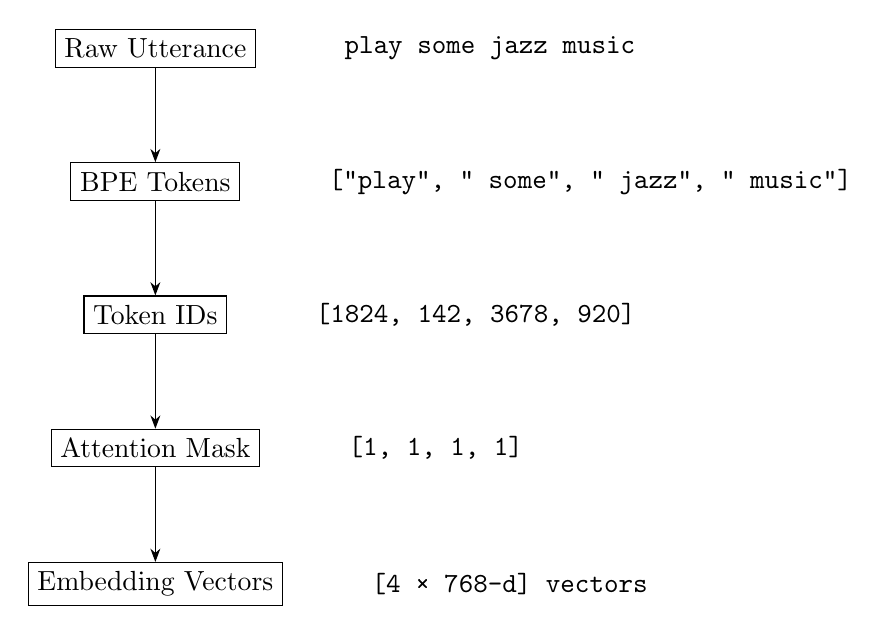
\begin{tikzpicture}[node distance=1.2cm]
    \node[draw, rectangle] (text) {Raw Utterance};
    \node[draw, rectangle, below=of text] (tokens) {BPE Tokens};
    \node[draw, rectangle, below=of tokens] (ids) {Token IDs};
    \node[draw, rectangle, below=of ids] (mask) {Attention Mask};
    \node[draw, rectangle, below=of mask] (embed) {Embedding Vectors};

    \draw[-Stealth] (text) -- (tokens);
    \draw[-Stealth] (tokens) -- (ids);
    \draw[-Stealth] (ids) -- (mask);
    \draw[-Stealth] (mask) -- (embed);

    \node[right=1cm of text] {\texttt{play some jazz music}};
    \node[right=1cm of tokens] {\texttt{["play", " some", " jazz", " music"]}};
    \node[right=1cm of ids] {\texttt{[1824, 142, 3678, 920]}};
    \node[right=1cm of mask] {\texttt{[1, 1, 1, 1]}};
    \node[right=1cm of embed] {\texttt{[4 × 768-d] vectors}};
 \end{tikzpicture}
\end{frame}



% Slide 8: Training Progress (Previously Slide 7)
\begin{frame}
\frametitle{Training Progress}
\begin{columns}
  \column{0.5\textwidth}
  \textbf{Loss and Metrics Tracking}
  \begin{itemize}
    \item Training loss decreases steadily
    \item Validation metrics show convergence
    \item No significant overfitting observed
    \item Full-model fine-tuning shows better convergence
  \end{itemize}

  \column{0.5\textwidth}
  \begin{figure}
     \includegraphics[width=\textwidth]{last-linear-layer/accuracy_metrics.png}
     \caption{Example: Accuracy over Epochs}
  \end{figure}
\end{columns}
\end{frame}

% New Slide 8: Training and Dev Loss (Previously Slide 7)
\begin{frame}
\frametitle{Training and Development Loss}
\centering
\begin{figure}
  \includegraphics[width=0.9\textwidth]{last-linear-layer/loss_metrics.png}
  \caption{Training and Development Loss over Epochs}
\end{figure}
\end{frame}

% New Slide 9: Accuracy over Epochs (Previously Slide 8)
\begin{frame}
\frametitle{Accuracy over Epochs}
\centering
\begin{figure}
  \includegraphics[width=0.9\textwidth]{last-linear-layer/accuracy_metrics.png}
  \caption{Accuracy Performance over Epochs (Last-Linear-Layer)}
\end{figure}
\end{frame}

% New Slide 10: Fine-tuning Mode Accuracy Comparison (Previously Slide 9)
\begin{frame}
\frametitle{Accuracy Comparison: Last-Linear-Layer vs. Full-Model}
\centering
\begin{columns}
  \column{0.48\textwidth}
  \begin{figure}
    \includegraphics[width=\textwidth]{last-linear-layer/accuracy_metrics.png}
    \caption{Last-Linear-Layer Accuracy}
  \end{figure}
  \column{0.48\textwidth}
  \begin{figure}
    \includegraphics[width=\textwidth]{full-model/accuracy_metrics.png}
    \caption{Full-Model Accuracy}
  \end{figure}
\end{columns}
\end{frame}

\begin{frame}
  \frametitle{F1 Score Comparison: Last-Linear-Layer vs. Full-Model}
  \centering
  \begin{columns}
    \column{0.48\textwidth}
    \begin{figure}
      \includegraphics[width=\textwidth]{last-linear-layer/f1_metrics.png}
      \caption{Last-Linear-Layer F1 Scores}
    \end{figure}
    \column{0.48\textwidth}
    \begin{figure}
      \includegraphics[width=\textwidth]{full-model/f1_metrics.png}
      \caption{Full-Model F1 Scores}
    \end{figure}
  \end{columns}
\end{frame}

\begin{frame}
  \frametitle{Comparison to Official MASSIVE Benchmark (EN-US)}
  
  \textbf{Intent Accuracy on EN-US Subset:} \\[0.5em]
  \href{https://arxiv.org/pdf/2204.08582}{\texttt{FitzGerald et al., 2022 (arXiv:2204.08582)}}
    
  \begin{tabular}{lcc}
    \toprule
    \textbf{Model} & \textbf{Type} & \textbf{Accuracy (\%)} \\
    \midrule
    \textbf{GPT-2} & Decoder-only (monolingual) & \textbf{80.1} \\
    mT5 Enc Full & Encoder-decoder (multilingual) & 89.0 ± 1.1 \\
    mT5 T2T Full & Encoder-decoder (multilingual) & 87.9 ± 1.2 \\
    XLM-R Full & Encoder-only (multilingual) & 88.3 ± 1.2 \\
    \bottomrule
  \end{tabular}
    
  \vspace{1em}
  \textbf{Interpretation:}
  \begin{itemize}
    \item Our GPT-2 model achieves \textbf{competitive performance} without cross-lingual supervision.
    \item Models in the paper use \textbf{larger pretraining corpora}, \textbf{multilingual tokens}, and more parameters.
  \end{itemize}
    
  \textit{→ For an English-only GPT-2 baseline, 80\% accuracy is strong given the task complexity.}
\end{frame}

\begin{frame}
  \frametitle{Ours vs. Original MASSIVE Benchmark}
  
  \textbf{Original MASSIVE Benchmark (FitzGerald et al., 2022)} \\[0.5em]
  \href{https://arxiv.org/pdf/2204.08582}{\texttt{arXiv:2204.08582}}
  
  \vspace{0.5em}
  \begin{itemize}
    \item mT5 / XLM-R models trained using:
    \begin{itemize}
      \item \texttt{p3dn.24xlarge} (8x V100 GPUs) for 3–5 days
      \item \texttt{g4dn.metal} (8x T4 GPUs) for mT5 Encoder
      \item Extensive hyperparameter tuning on multilingual data
    \end{itemize}
  \end{itemize}
  
  \vspace{1em}
  \textbf{Our Setup (GPT-2):}
  \begin{itemize}
    \item Single \texttt{RTX 3080} GPU
    \item Training time: \textbf{~3 hours total}
    \item No multilingual pretraining or zero-shot setup
  \end{itemize}
  
  \vspace{1em}
  \textbf{Conclusion:} Our monolingual GPT-2 model achieves competitive performance with only a fraction of the computational cost.
\end{frame}

\end{document}


